
C++ 中最引人注目的功能之一是代码的重用,
当然这意味着不仅仅是对代码进行简单的复制和更改。
如何更好的实现代码的重用?
这与 C++ 中的大多数内容一样,解决方案围绕类(class)。 
我们可以通过创建新的类来重用代码,
但是可以使用其他人已经构建和调试的现有类,
而不是从头开始创建它们。
其优势在于我们可以不污染现有代码的前提下使用这些新的类。

实现代码重用的两个有效手段是
继承(inheritance)和组合(composition)。
组合是指新类中的成员是另一个或多个现有类的对象。
之所以称为组合,是因为新类是由现有类的对象组成。
更普遍的说,是 has-a 的关系,
例如汽车具有(has-a)引擎(见图 \ref{fig:has-a})。
\begin{figure}[htbp]
  \centering
  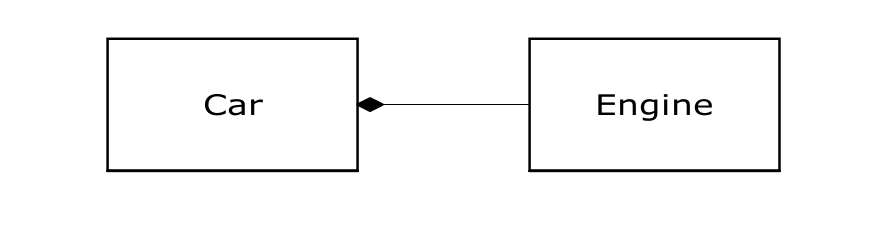
\includegraphics[width=0.5\textwidth]{png/has-a}
  \caption{C++ 中 has-a 的关系。}
  \label{fig:has-a}
\end{figure}
组合具有很大的灵活性。
因为新类的成员对象通常是私有的,
这使得使用该类的客户端程序员无法访问它们。
这方便让我们更改那些成员而不会打扰现有的客户端代码。
同时由于其简单,灵活,我们在程序设计中应该首先考虑。

继承是直接采用现有类的形式并向其中添加代码,而无需修改现有类。
如果更改了原始类(称为基类或者父类),
则继承后的类(称为派生类或者子类)也反映了这些变化。
这两种类型可以具有共同的特征和行为,
同时一种类型可能比另一种包含更多特征并且还可以处理更多消息。
我们也称之为 is-a 的关系。
图 \ref{fig:is-a} 是计算机辅助设计中经常遇见的形状案例。
基本类型是形状,每个形状都有大小,颜色,位置,
并且可以绘制,删除,移动,着色等,
从中派生特定类型的形状:圆形,正方形,三角形等,
每种形状可能具有其他特征和行为。 
例如,当你要计算形状的面积时,某些行为可能会有所不同。
\begin{figure}[htbp]
	\centering
	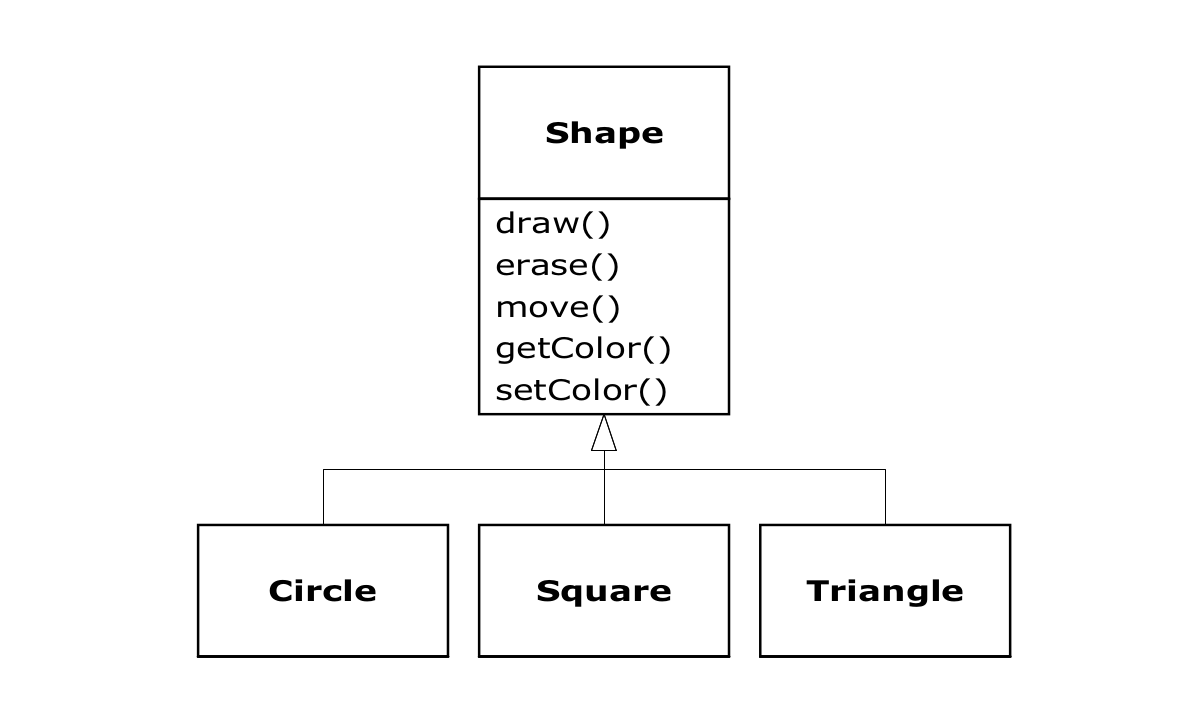
\includegraphics[width=0.5\textwidth]{png/is-a}
	\caption{C++ 中 is-a 的关系。}
	\label{fig:is-a}
\end{figure}

在这里我们只是强调一下这两个概念的重要性
而不去过多的解读它们。
如果你想系统的学习 C++,可以参考书籍
\begin{itemize}
	\item Thinking in C++, Volume 1: Introduction to Standard C++
		\cite{eckel2000thinking};
	\item Thinking in C++, Volume 2 : Practical Programming
		\cite{eckel2004thinking}。
\end{itemize}

\begin{remark}
	因为继承和组合在面向对象的编程中非常重要,
	我们这里不得不单独列一小结去高度强调它。
	在程序设计的时候应该首先考虑这两种关系,
	合理的运用,会使我们的设计更加简洁,灵活。
	但切记盲目使用,学会在实战中寻找经验!
\end{remark}






%%% Local Variables:
%%% mode: latex
%%% TeX-master: "../Guide"
%%% End:
